\documentclass[journal]{IEEEtran}
\usepackage{amsmath,amssymb,amsthm}
\usepackage{booktabs}
\usepackage{cite}
\usepackage{url}
\usepackage[hidelinks]{hyperref}
\usepackage{tikz}
\usetikzlibrary{positioning,arrows.meta}

\newtheorem{proposition}{Proposition}
\newtheorem{theorem}{Theorem}
\newtheorem{corollary}{Corollary}
\newtheorem{lemma}{Lemma}
\newcommand{\eps}{\varepsilon}

\begin{document}

\title{Private Flow Matching for Tabular Data: An Optimal-Transport Pitfall, a Certified Audit, and Why Marginals Do the Work}

\author{Author~Name,~\IEEEmembership{Member,~IEEE}% <-- fill in
\thanks{Manuscript draft, September 2026. Code and all raw results: \url{<artifact URL>}.}}

\maketitle

\begin{abstract}
We study differentially private (DP) tabular data synthesis with flow matching trained by DP-SGD, and report three findings.

\emph{First, a privacy pitfall.} Minibatch optimal-transport (OT) couplings, a popular way to straighten flows, make each example's loss depend on the whole batch. This silently voids the per-example sensitivity bound that DP-SGD's accountant relies on. We prove the failure, and we prove that independent coupling (I-CFM) satisfies the bound by construction. On UCI Adult, an adversarial replacement record re-pairs up to 26 of 64 batch members and raises the clipped-gradient-sum sensitivity to $1.18\times$ the assumed bound; on a 20k-row cardiovascular dataset the bound is exceeded in 69\% of batches, by up to $1.48\times$. White-box audits certify, at 95\% confidence, that any valid certificate must state $\eps\ge0.898$ (Adult) and $\eps\ge1.47$ (Cardio) where $0.735$ and $0.839$ were reported.

\emph{Second, a sound pipeline.} We give an end-to-end $(\eps,\delta)$ proof for a complete public-schema synthesis pipeline built on I-CFM. The pipeline has a data-independent budget controller (DAPC) and a DP class-conditional marginal stage, composed with DP-SGD in a single PRV accountant. Formalising the proof against the code exposed five further leak classes, which we give as a checklist.

\emph{Third, a negative result about where utility comes from.} With the marginal stage, test AUC on Adult rises from $0.49$ to $0.906$ at $\eps=0.741$, above AIM ($0.790$) and MST ($0.713$), and a 20k-row cardiovascular dataset reaches the real-data ceiling. However, removing the flow entirely leaves every metric statistically equivalent (10 paired seeds, TOST $p<0.001$ at margins $\pm0.01$ AUC and $\pm0.005$ TVD), and the same holds at every $\eps\le4.7$ tested. The best budget split gives $\ge90\%$ of $\eps$ to the marginals. At practical privacy levels, the DP-SGD-trained flow contributes no measurable value; the DP marginals do the work.
\end{abstract}

\begin{IEEEkeywords}
Differential privacy, DP-SGD, flow matching, optimal transport, privacy auditing, synthetic data, negative results.
\end{IEEEkeywords}

\section{Introduction}
\IEEEPARstart{D}{eep} generative models trained with DP-SGD~\cite{abadi2016deep} are a common route to private synthetic data, and flow matching~\cite{lipman2023flow,liu2023flow} is a natural candidate: it trains stably and samples quickly. This paper examines the route end to end on tabular data and reports three findings: one about privacy, one about soundness, and one about utility.

\textbf{A privacy pitfall.} DP-SGD's guarantee rests on one invariant: each example influences the noised gradient only through its own clipped gradient. Minibatch OT couplings (OT-CFM)~\cite{tong2024improving,pooladian2023multisample} pair noise and data by solving an assignment over the whole batch, which breaks the invariant. The accountant keeps reporting the same $\eps$, because it reads only the noise multiplier, the sampling rate and the number of steps. The general phenomenon, that non-decomposable losses have batch-size-dependent sensitivity, is known for contrastive losses~\cite{kong2025nondecomposable} and batch normalisation~\cite{yousefpour2021opacus}. We are not aware of prior work identifying it for OT couplings in generative training, or quantifying it with a certified audit.

\textbf{A sound pipeline.} We build a complete DP tabular synthesiser on I-CFM and prove its release guarantee against the code, not only against the design. Doing so exposed five further leaks, none of which changes the reported $\eps$.

\textbf{Where utility comes from.} At $\eps<1$ the flow alone performs at chance on downstream tasks. A budget split that spends part of $\eps$ on DP class-conditional marginals, following the MST/AIM recipe~\cite{mckenna2021winning,mckenna2022aim}, raises utility to AIM's level or above. The ablation that matters, however, is marginals \emph{without} the flow: it matches every configuration. We report this negative result explicitly, because the natural reading of such a pipeline credits the deep model.

\textbf{Contributions.}
\begin{enumerate}
\item A proof that batch-OT coupling voids DP-SGD's sensitivity bound under both add/remove and replace-one adjacency, and that I-CFM restores it (Section~\ref{sec:pitfall}).
\item A real-data counterexample and a certified white-box audit on two datasets, showing the reported $\eps$ understates the smallest valid certificate by 22\% (Adult) and 76\% (Cardio) (Section~\ref{sec:audit}).
\item An end-to-end proof for a public-schema pipeline with a data-independent budget controller and a jointly accounted DP marginal stage, plus a five-item leak checklist (Sections~\ref{sec:pipeline}--\ref{sec:lessons}).
\item A controlled utility study across three datasets and $\eps\in[0.74,4.7]$, with matched-$\eps$ baselines. DP marginals deliver all measurable utility, and the DP-SGD flow adds none (Section~\ref{sec:utility}).
\end{enumerate}

\section{Background}
\subsection{Differential privacy and DP-SGD}
A randomised mechanism $\mathcal M$ is $(\eps,\delta)$-DP if $\Pr[\mathcal M(D)\in S]\le e^\eps\Pr[\mathcal M(D')\in S]+\delta$ for all neighbouring $D\simeq D'$ and all events $S$~\cite{dwork2006calibrating}. We use add/remove adjacency. DP-SGD samples a Poisson batch $B$ with rate $q$, clips every per-example gradient to norm $C$, and releases $S(B)+\mathcal N(0,\sigma^2C^2I)$ with $S(B)=\sum_{i\in B}\bar g_i$. Accountants (RDP~\cite{mironov2017renyi}, PRV~\cite{gopi2021numerical}) compose steps under the assumption $\|S(B)-S(B')\|_2\le C$, or $2C$ under replace-one adjacency.

\subsection{Gaussian differential privacy}
A Gaussian step with sensitivity $\Delta$ and noise $\sigma C$ is $(\Delta/\sigma C)$-GDP~\cite{dong2022gaussian}. For any test with rates $(\alpha,\beta)$ against a $\mu$-GDP mechanism, $\mu\ge\Phi^{-1}(1-\alpha)-\Phi^{-1}(\beta)$. This yields valid lower bounds from Monte-Carlo estimates~\cite{nasr2023tight}.

\subsection{Flow matching and couplings}
Conditional flow matching regresses $v_\theta(z_t,t)$ onto $z_1-z_0$ along $z_t=(1-t)z_0+tz_1$~\cite{lipman2023flow}. \emph{I-CFM} pairs $z_{0,i}$ with $z_{1,i}$ independently. \emph{OT-CFM} solves $\pi^\star=\arg\min_\pi\sum_i\|z_{0,i}-z_{1,\pi(i)}\|^2$ over the batch~\cite{kuhn1955hungarian,tong2024improving}.

\section{Threat Model}\label{sec:threat}
The adversary knows the code, every hyper-parameter, the public schema and every record except the target's, and may choose the neighbouring dataset. It observes the synthetic dataset, the released network weights and the privacy summary. Training telemetry is computed without noise and is not released. We assume:
\begin{itemize}
\item[A1] a public schema of types, bounds and categories;
\item[A2] a public cohort size $N$, as in every DP-SGD deployment that sets $q=B/N$;
\item[A3] public column and target names;
\item[A4] unpredictable noise (floating-point attacks~\cite{mironov2012lsb} are out of scope).
\end{itemize}
A2 matters beyond sampling: dividing the noisy sum by the expected batch size $qN$ is post-processing only if $N$ is public, a subtlety recently shown to affect deployed implementations~\cite{wang2026rethinking}.

\section{The Pitfall}\label{sec:pitfall}
\begin{proposition}[I-CFM respects DP-SGD's bound]\label{prop:icfm}
Under I-CFM, $\ell_i$ depends only on $(z_{0,i},z_{1,i},t_i,\theta)$ with per-example independent $z_{0,i},t_i$. Adding or removing record $j$ therefore changes $S(B)$ by exactly $\bar g_j$, so $\|S(B)-S(B')\|_2\le C$.
\end{proposition}

\begin{theorem}[Batch-OT voids it]\label{thm:ot}
Under OT-CFM, changing record $j$ may re-pair a set $R$ of other records, $|R|=k\le|B|-1$. Then $\|S(B)-S(B')\|_2=\|\sum_{i\in\{j\}\cup R}(\bar g_i(B)-\bar g_i(B'))\|_2\le2C(k+1)$, and DP-SGD's bound is not guaranteed. One violating pair suffices, since DP is a worst-case property.
\end{theorem}

\begin{corollary}
A replace-one violation ($>2C$) implies, by the triangle inequality through $B\setminus\{j\}$, an add/remove violation ($>C$). OT-CFM breaks the bound under either adjacency.
\end{corollary}

This is an instance of the non-decomposable-loss problem~\cite{kong2025nondecomposable}. Here, however, the coupling rather than the loss creates the dependence, and the loss itself looks per-example.

\section{Empirical Audit}\label{sec:audit}
\textbf{Setup.} UCI Adult~\cite{becker1996adult}: 15{,}000 rows, public-schema encoding to $d=78$. The velocity network is an MLP with 128 hidden units and LayerNorm. Batches have 64 records, over 10 initialisations $\times$ 10 batches, with replace-one neighbours; we report $\Delta/2C$. $C$ is set so that every gradient is clipped, as in all our training runs.

\textbf{Sensitivity.} We use three adversaries of increasing strength (Table~\ref{tab:sens}):
\begin{itemize}
\item \emph{random}: a random real record;
\item \emph{screened}: the best of 313 candidates by the number of records they re-pair;
\item \emph{hill-climbed}: screened candidates restricted to valid records and then locally optimised.
\end{itemize}
Under the screened adversary, one replacement re-pairs 13.9 records on average (maximum 26).

\begin{table}[t]\centering\caption{Clipped-sum sensitivity $\Delta/2C$ (100 batches per row). Cardio: 20k rows, $d=12$.}\label{tab:sens}
\begin{tabular}{lcccc}\toprule
& \multicolumn{2}{c}{Batch-OT} & \multicolumn{2}{c}{I-CFM}\\
adversary & max & $>1$ & max & $>1$\\\midrule
Adult, random & 0.99 & 0\% & 0.54 & 0\%\\
Adult, screened & 1.147 & 15\% & 0.648 & 0\%\\
Adult, hill-climbed & \textbf{1.182} & \textbf{17\%} & 0.681 & 0\%\\
Cardio, hill-climbed & \textbf{1.484} & \textbf{69\%} & 0.975 & 0\%\\\bottomrule
\end{tabular}\end{table}

\textbf{White-box step audit.} For the worst pair, we run the real Gaussian mechanism $10^6$ times per hypothesis, with the training $\sigma=2.617$ and full-dimensional noise. We apply the Neyman--Pearson test and Clopper--Pearson bounds~\cite{clopper1934} (Bonferroni, 95\%). The audit gives $\mu\ge0.896$ against a claimed $2/\sigma=0.764$ (Table~\ref{tab:audit}). Re-accounting with effective noise $\sigma\mu_{claim}/\mu_{lb}$, no valid certificate for the OT run can state $\eps<0.898$, yet $0.735$ was reported. I-CFM's worst pair gives $\mu\ge0.518$, consistent with its guarantee. On Cardio the violation is larger and more frequent: $\mu\ge1.427$ against $0.966$, so the minimum valid certificate is $\eps\ge1.474$ against a reported $0.839$, while I-CFM stays within its bound ($0.975\times$ in the worst case).

\begin{table}[t]\centering\caption{Certified white-box audits of one DP-SGD step ($10^6$ trials per hypothesis).}\label{tab:audit}
\begin{tabular}{lcc}\toprule
 & Batch-OT & I-CFM\\\midrule
\multicolumn{3}{l}{\emph{Adult} ($\sigma=2.617$)}\\
$\mu$ lower bound (95\%) / claimed & \textbf{0.896} / 0.764 & 0.518 / 0.764\\
reported / min.\ valid $\eps$ & 0.735 / \textbf{0.898} & 0.735 / 0.735\\
\multicolumn{3}{l}{\emph{Cardio} ($\sigma=2.070$)}\\
$\mu$ lower bound (95\%) / claimed & \textbf{1.427} / 0.966 & 0.936 / 0.966\\
reported / min.\ valid $\eps$ & 0.839 / \textbf{1.474} & 0.839 / 0.839\\\bottomrule
\end{tabular}\end{table}

\textbf{Black-box audit.} We also ran a one-run canary audit~\cite{steinke2023one} on the synthetic data. It has no power here: $\eps_{lb}=0$ for every run, including a near-non-private control ($\eps=28.6$). Implementation-level violations of this kind are visible only white-box~\cite{tramer2022debugging}.

\section{A Sound Pipeline}\label{sec:pipeline}
The pipeline (Fig.~\ref{fig:pipeline}) has five parts:
\begin{enumerate}
\item public-schema preprocessing, which is row-local;
\item \emph{DAPC}, which selects $\eps^\star$ and the budget split from public metadata;
\item DP-SGD training of an I-CFM velocity field;
\item optional \emph{Stage 7c}: noisy class-conditional marginals;
\item post-processing: sampling, public-domain repair, and within-class quantile mapping onto the noisy marginals, with the flow's within-class ranks kept as the copula.
\end{enumerate}

\begin{figure}[t]\centering
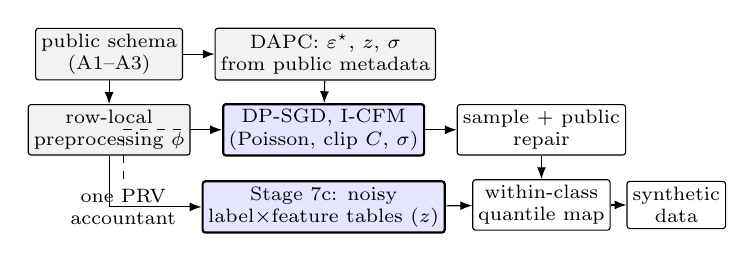
\begin{tikzpicture}[font=\scriptsize, node distance=3mm and 4mm,
  box/.style={draw, rounded corners=1pt, align=center, minimum height=6mm, inner sep=2pt},
  pub/.style={box, fill=gray!10}, dp/.style={box, fill=blue!10, thick}, arr/.style={-{Latex[length=1.5mm]}}]
\node[pub] (schema) {public schema\\(A1--A3)};
\node[pub, right=of schema] (dapc) {DAPC: $\eps^\star$, $z$, $\sigma$\\from public metadata};
\node[pub, below=of schema] (pre) {row-local\\preprocessing $\phi$};
\node[dp, right=of pre] (sgd) {DP-SGD, I-CFM\\(Poisson, clip $C$, $\sigma$)};
\node[dp, below=of sgd] (cm) {Stage 7c: noisy\\label$\times$feature tables ($z$)};
\node[box, right=of sgd] (samp) {sample + public\\repair};
\node[box, below=of samp] (recal) {within-class\\quantile map};
\node[box, right=of recal, xshift=-2mm] (out) {synthetic\\data};
\node[left=of cm, align=center, xshift=2mm] (acc) {one PRV\\accountant};
\draw[arr] (schema) -- (pre); \draw[arr] (schema) -- (dapc); \draw[arr] (pre) -- (sgd);
\draw[arr] (dapc) -- (sgd); \draw[arr] (pre) |- (cm); \draw[arr] (sgd) -- (samp);
\draw[arr] (samp) -- (recal); \draw[arr] (cm) -- (recal); \draw[arr] (recal) -- (out);
\draw[dashed] (acc) -- (cm); \draw[dashed] (acc.north) |- (sgd.west);
\end{tikzpicture}
\caption{Pipeline. Shaded blue: the only mechanisms that touch private data; both are Gaussian and composed in a single PRV accountant. Grey: functions of public information only. Everything downstream is post-processing.}\label{fig:pipeline}
\end{figure}

\begin{lemma}[Row-local preprocessing]
Under A1, preprocessing applies a fixed map $\phi$ to each record, so $D\simeq D'\Rightarrow\phi(D)\simeq\phi(D')$.
\end{lemma}

\begin{lemma}[Stage 7c]
$M$ tables of shape (label levels $\times$ feature levels) on public bins have add/remove $\ell_2$-sensitivity $\sqrt M$. Adding $\mathcal N(0,z^2M)$ per cell is a Gaussian mechanism with noise multiplier $z$. It is recorded in the same PRV accountant as the DP-SGD steps, and the flow's $\sigma$ is calibrated so that the joint composition equals $\eps^\star$.
\end{lemma}

\begin{lemma}[DAPC is free]
$\eps^\star$, the marginal noise $z$ and $\sigma$ are deterministic functions of public $(N,d,$ name-based scores, target name, $K, M)$, fixed before any mechanism runs.
\end{lemma}

\begin{theorem}[End-to-end]
Under A1--A4, the release is $(\eps^\star,\delta)$-DP with respect to add/remove adjacency. The run asserts that the accountant is within target before releasing.
\end{theorem}
\begin{proof}[Proof sketch]
Public stages and DAPC are constants. DP-SGD with I-CFM is a subsampled Gaussian mechanism by Proposition~\ref{prop:icfm}, and the accountant's $q=B/N$ bounds the loader's rate from above. Stage 7c is a Gaussian mechanism with independent noise, composed in the same PRV accountant. Everything else is post-processing. The full proof, with every code path classified, is in the artifact.
\end{proof}

\section{Lessons: Five Further Leak Classes}\label{sec:lessons}
Proving the guarantee against the code exposed five further leaks in our implementation. All are fixed and covered by regression tests:
\begin{enumerate}
\item fixed seeds on noise paths, which make the noise subtractable;
\item clipping the noise instead of the query;
\item an un-noised feature-similarity graph over private rows, stored as a buffer of the released network;
\item a histogram bin edge set to the smallest private value;
\item silent schema fallback to private minima, maxima and categories.
\end{enumerate}
None changes the reported $\eps$, so none is visible from the privacy summary.

\section{Utility: Where It Comes From}\label{sec:utility}
\textbf{Protocol.} We use three datasets:
\begin{itemize}
\item Adult (12k training rows, TRTR AUC 0.917);
\item Cardio (a 20k-row sample of the Kaggle cardiovascular dataset, clinically plausible public bounds, TRTR 0.779);
\item Pima (614 rows, TRTR 0.812).
\end{itemize}
The target is $\eps=1$, and DAPC selects $\eps^\star=0.741$, $0.849$ and $0.753$ respectively. TSTR is the AUC of a random forest trained on synthetic data and tested on a real holdout. TVD is the mean total variation of 1-way and all 2-way marginals on public bins. Each cell averages 3 seeds, and every run passed the accountant check.

\textbf{Coupling.} I-CFM vs.\ OT on Adult (10 paired seeds, flow only): TSTR $0.533\pm0.049$ vs.\ $0.526\pm0.091$, Wilcoxon $p=0.49$. The sound coupling costs nothing detectable, but both are at chance.

\textbf{Budget split and the decisive ablation.} Table~\ref{tab:split} varies the share of $\eps$ spent on Stage 7c and removes the flow (``marginals only'': within-class ranks drawn at random instead of taken from the flow). Utility rises monotonically with the marginal share. Marginals-only matches the full pipeline everywhere. With 10 paired seeds at share 0.9, the two are statistically equivalent: TSTR differences are $-0.0001$ (Adult, 95\% CI $[-0.0023,0.0021]$) and $-0.0004$ (Cardio, $[-0.0038,0.0030]$), with TOST $p<0.001$ at a $\pm0.01$ margin. The one detectable effect of the flow is a 0.0011 reduction in Cardio's 2-way TVD (Wilcoxon $p=0.01$), about 2\% of the error and well inside the equivalence margin. The same holds at $\eps^\star=2.45$ and $4.72$ on Adult (full $0.905/0.906$ vs.\ marginals-only $0.906/0.907$; flow alone $0.526/0.581$). The DP-SGD flow contributes no measurable value, and noise multiplicity~\cite{dockhorn2023dpdm} with a smaller network does not change this.

\begin{table}[t]\centering\caption{Budget split and flow ablation (TSTR AUC / 2-way TVD).}\label{tab:split}
\setlength{\tabcolsep}{3pt}
\begin{tabular}{lccc}\toprule
config & Adult & Cardio & Pima\\\midrule
flow only & 0.492 / 0.719 & 0.732 / 0.365 & 0.514 / 0.795\\
flow + 1-way marginals & 0.497 / 0.271 & 0.710 / 0.227 & 0.477 / 0.773\\
share 0.2 & 0.879 / 0.207 & 0.775 / 0.082 & 0.696 / 0.736\\
share 0.6 & 0.901 / 0.114 & 0.780 / 0.049 & 0.768 / 0.590\\
DAPC adaptive split & 0.904 / 0.116 & 0.780 / 0.070 & 0.729 / 0.601\\
share 0.9 (10 seeds) & \textbf{0.906} / 0.096 & 0.779 / \textbf{0.044} & --\\
share 0.9, \emph{marginals only} (10 seeds) & 0.906 / \textbf{0.095} & 0.779 / 0.046 & --\\\bottomrule
\end{tabular}\end{table}

\textbf{Matched-$\eps$ baselines.} On Adult at $\eps=0.741$ (Table~\ref{tab:base}), the pipeline with Stage 7c exceeds AIM~\cite{mckenna2022aim} and MST~\cite{mckenna2021winning} on TSTR, and matches or beats them on 2-way TVD. Deep baselines~\cite{rosenblatt2020dpsynth,jordon2019pategan,xu2019ctgan}, and our flow without marginals, are at chance. Stage 7c is \emph{target-aware}. For a fair comparison we also give AIM only the label$\times$feature workload: its TSTR rises to $0.872$ but stays below ours, and its 2-way TVD degrades to $0.267$.

\begin{table}[t]\centering\caption{Adult, $\eps=0.741$, $\delta=10^{-5}$, 3 seeds.}\label{tab:base}
\begin{tabular}{lccc}\toprule
method & TSTR AUC & 1-way TVD & 2-way TVD\\\midrule
ours, share 0.9 & $\mathbf{0.906\pm0.002}$ & 0.029 & \textbf{0.097}\\
AIM, label$\times$feature workload & $0.872\pm0.002$ & 0.015 & 0.267\\
AIM & $0.790\pm0.011$ & 0.018 & 0.112\\
MST & $0.713\pm0.031$ & \textbf{0.014} & 0.128\\
PATE-CTGAN & $0.534\pm0.043$ & 0.506 & 0.705\\
ours, flow only & $0.492\pm0.054$ & 0.510 & 0.719\\
DP-CTGAN & $0.484\pm0.036$ & 0.298 & 0.468\\\bottomrule
\end{tabular}\end{table}

\textbf{Small cohorts.} Without Stage 7c, the flow is at chance on all four small datasets (455--1600 rows, 5 seeds) under every schedule tried. Some means fall below chance, such as Wisconsin's $0.31\pm0.15$. These are random-initialisation artifacts, not signal: the same seed gives AUC $\approx0.1$ even at $\eps=50$.

\textbf{DAPC.} The $\eps^\star$ selection is stable under joint perturbation of its hand-set constants (2000 draws; median Kendall $\tau=0.96$; $\le0.011$ change for a $+10\%$ change to any single weight). The adaptive split rule, which targets a relative cell noise and caps at a 0.6 share, matches the best fixed split on Adult but not on Cardio (TVD 0.070 vs.\ 0.044). The evidence favours simply giving most of the budget to the marginals. An adaptive allocator has nothing to allocate between while the second mechanism earns no budget.

\section{Related Work}
\textbf{DP-SGD correctness and auditing.} Non-decomposable losses~\cite{kong2025nondecomposable}, batch statistics~\cite{yousefpour2021opacus} and normalisation by batch size~\cite{wang2026rethinking} all break or weaken DP-SGD's analysis. Auditing lower-bounds $\eps$ and has found real bugs~\cite{jagielski2020auditing,nasr2021adversary,nasr2023tight,steinke2023one,tramer2022debugging}. We add OT couplings to this list, with a certified audit.

\textbf{DP generative models.} Relevant work includes DP diffusion~\cite{dockhorn2023dpdm}, DP rectified flow for images, which likewise spends part of the budget on class-conditional statistics~\cite{che2026straightdp}, DP GANs~\cite{jordon2019pategan,rosenblatt2020dpsynth}, and marginal-based synthesisers~\cite{mckenna2021winning,mckenna2022aim}, which dominate tabular benchmarks~\cite{tao2021benchmarking}. Our negative result is consistent with that benchmark evidence and sharpens it: even when paired with strong DP marginals, the deep component adds nothing at $\eps\le4.7$.

\section{Limitations}
\begin{itemize}
\item Configuration sweeps use 3 seeds per cell; the headline equivalence and the coupling comparison use 10 paired seeds.
\item Stage 7c is target-aware; multi-task use would need a workload over several targets.
\item The flow might contribute with public pretraining or at much larger $N$, which we did not test.
\item Assumption A2 and the use of non-cryptographic PRNGs are stated caveats.
\item HVAE mode is excluded from all claims.
\end{itemize}

\section{Conclusion}
Minibatch OT coupling silently invalidates DP-SGD's accounting; independent coupling restores a provable guarantee at no detectable cost. Proving a synthesis pipeline against its code, not its design, exposed five further leaks that no privacy summary could reveal. Finally, at practical privacy levels the DP-SGD flow is not where utility comes from: jointly accounted DP marginals deliver all of it, and a pipeline without the flow performs identically. We recommend that DP generative papers report this ablation as a matter of course.

\bibliographystyle{IEEEtran}
\bibliography{refs}
\end{document}
